%!TEX TS-program = xelatex
\documentclass[]{friggeri-cv}
\usepackage{afterpage}
\usepackage{hyperref}
\usepackage{color}
\usepackage{xcolor}
\usepackage{smartdiagram}
\usepackage{fontspec}
% if you want to add fontawesome package
% you need to compile the tex file with LuaLaTeX
% References:
%   http://texdoc.net/texmf-dist/doc/latex/fontawesome/fontawesome.pdf
%   https://www.ctan.org/tex-archive/fonts/fontawesome?lang=en
%\usepackage{fontawesome}
\usepackage{metalogo}
\usepackage{dtklogos}
\usepackage[utf8]{inputenc}
\usepackage{tikz}
\usepackage{enumitem}
\usetikzlibrary{mindmap,shadows}
\hypersetup{
    pdftitle={Jean-Romain Pr\'{e}vost - Senior Software Engineer},
    pdfauthor={Jean-Romain Pr\'{e}vost},
    pdfsubject={Resume},
    pdfkeywords={Senior Software Engineer, React, TypeScript, JavaScript, AI, Meta},
    colorlinks=true,           % no link border color
    allbordercolors=white,      % white border color for all
    pdfborderstyle={/S/U/W 0.8}, % optional: underline instead
}
\smartdiagramset{
    bubble center node font = \footnotesize,
    bubble node font = \footnotesize,
    % specifies the minimum size of the bubble center node
    bubble center node size = 0.35cm,
    %  specifies the minimum size of the bubbles
    bubble node size = 0.5cm,
    % specifies which is the distance among the bubble center node and the other bubbles
    distance center/other bubbles = 0.4cm,
    % sets the distance from the text to the border of the bubble center node
    distance text center bubble = 0.4cm,
    % set center bubble color
    bubble center node color = lightpink,
    % define the list of colors usable in the diagram
    set color list = {materialcyan, materiallime, materialamber, materialteal, materialindigo, materialgreen, orange, materialorange, green, lightgray},
    % sets the opacity at which the bubbles are shown
    bubble fill opacity = 0.6,
    % sets the opacity at which the bubble text is shown
    bubble text opacity = 0.8,
}

\addbibresource{bibliography.bib}
\RequirePackage{xcolor}
\definecolor{pblue}{HTML}{EE4466}

\begin{document}
\header{Jean-Romain} {Pr\'{e}vost}
      {Senior Software Engineer}
      
% Fake text to add separator      
\fcolorbox{white}{gray}{\parbox{\dimexpr\textwidth-2\fboxsep-2\fboxrule}{%
.....
}}

% In the aside, each new line forces a line break
\begin{aside}
    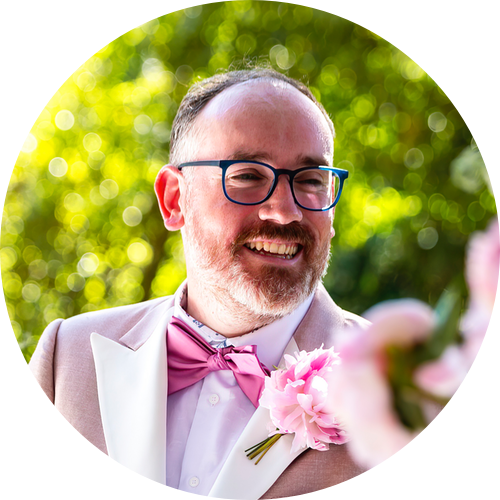
\includegraphics[scale=0.24]{img/cv-avatar-wedding.png}
  ~
  ~
  ~
  \section{Info}
        905 Laguna ave
        Burlingame
        94010 California
        ~
        (650) 422-4814
        ~
        \href{mailto:jr@ailleurs.me}{\textbf{jr@ailleurs.me}}
        \href{https://www.linkedin.com/in/jeanromain/}{\mbox{/in/jeanromain}}
        \href{https://github.com/3on}{github.com/3on}
  ~
  ~
  ~
  ~
% use  \hspace{} or \vspace{} to change bubble size, if needed
  \section{Skills}
    ~
    \smartdiagram[bubble diagram]{
        \textbf{JavaScript}\\\textbf{TypeScript},
        \textbf{React},
        \textbf{HTML5}\\\textbf{CSS3},
        \textbf{~Node.js~},
        \textbf{Python},
        \textbf{PHP},
        \textbf{GraphQL},
        \textbf{Next.js},
        \textbf{GenAI}
    }
\end{aside}

\section{Summary}
Senior Software Engineer with 12+ years of experience building consumer-facing web applications and developer tools at scale. Deep expertise in \textbf{React}, \textbf{TypeScript}, and the modern JavaScript ecosystem, with recent focus on \textbf{AI/ML product interfaces} at Meta.

\section{Experience}
\begin{entrylist}
    \entry
    {Aug 2025 - Present}
    {CTO / Co-Founder}
    {Tigo}
    {\begin{itemize}[nosep, leftmargin=1em, topsep=2pt]
        \item Co-founded \textbf{Tigo}, a tech-enabled marketplace connecting families with vetted in-home caregivers, targeting the \$160B+ U.S. home care market.
        \item Built the MVP end-to-end: a \textbf{Next.js}/\textbf{React} marketplace hosted on \textbf{Firebase} with \textbf{PostgreSQL} and \textbf{PostGIS} for geolocation features, styled with \textbf{Tailwind CSS}.
        \item Leveraged AI-assisted development (\textbf{Cursor}/\textbf{Claude}) to ship rapidly as a solo technical founder.
    \end{itemize}}

    \entry
    {Sep 2020 - Feb 2025}
    {Senior Software Engineer}
    {Meta}
    {\begin{itemize}[nosep, leftmargin=1em, topsep=2pt]
        \item Led development of a public-facing \textbf{AI image generation} playground (\href{https://about.fb.com/news/2023/12/meta-ai-updates/}{\texttt{imagine.meta.com}}) for the \textbf{Emu} launch. Delivered within a one-month deadline; at the time the only free image generation tool, attracting significant media attention and resharing by C-level executives.
        \item Maintained and developed various playgrounds within the \textbf{MetaGen} organization to support new \textbf{Llama} model releases and features, including \textbf{agent support}, side-by-side model comparisons, and file uploads.
        \item Created a debugging tool for \textbf{MetaGen} that tracks each step of the model request lifecycle, from prompt to final answer, highlighting changes to prompts and metadata throughout the process.
        \item Led front-end development for multiple \textbf{Meta Financial Technologies} (MFT) tools, improving internal adoption of new financial products.
        \item Contributed to bringing a \textbf{NFT wallet} viewer to \textbf{Facebook} and \textbf{Instagram} web.
        \item Maintained and modernized the \textbf{Facebook Stories} web viewer, ensuring a smooth Stories experience on \texttt{facebook.com}.
    \end{itemize}}

    \entry
    {Aug 2018 - Jan 2020}
    {Senior Frontend Engineer}
    {Cruise}
    {\begin{itemize}[nosep, leftmargin=1em, topsep=2pt]
        \item Contributed to a \textbf{React} web application enabling remote control and monitoring of \textbf{autonomous vehicles} as part of the Remote Assistance team.
        \item Improved tooling and test coverage by adding support for \textbf{Enzyme}, \textbf{Storybook}, and \textbf{Puppeteer}.
        \item Spearheaded rendering of the \textbf{WebGL} scene using the internal library \textbf{Worldview}.
    \end{itemize}}

    \entry
    {Sep 2014 - Mar 2018}
    {Software Engineer}
    {Yelp}
    {\begin{itemize}[nosep, leftmargin=1em, topsep=2pt]
        \item Modernized the web photos experience and led front-end for the web homepage redesign, both requiring complete front-end and back-end rewrites.
        \item Led front-end code packaging as part of the \textbf{micro-services} transition for the homepage project.
        \item Improved various components of the \textbf{iOS} business page: photo carousel header, search facet, bookmarks.
        \item Mentored interns and new hires; pushed code to production every other week.
    \end{itemize}}

    \entry
    {Jul 2013 - Sep 2014}
    {Frontend Engineer}
    {Montage Studio}
    {\begin{itemize}[nosep, leftmargin=1em, topsep=2pt]
        \item Built rich UI components for \textbf{Montage Studio}, a development tool for \textbf{Montage.js} applications, including a tree viewer and OS X-style context menus.
        \item Worked on a fully \textbf{JavaScript}-based stack (\textbf{Node.js} and Montage.js), a framework borrowing heavily from Cocoa's UI design patterns.
    \end{itemize}}
\end{entrylist}

\begin{entrylist}
    \entry
    {Jun 2013 - Oct 2013}
    {Open Source Contributor}
    {VideoLAN}
    {\begin{itemize}[nosep, leftmargin=1em, topsep=2pt]
        \item Submitted patches for the \textbf{VLC} \textbf{iOS} app as an open source contributor.
        \item Built a web application running on the phone that enables uploading content to the device via a built-in web server.
    \end{itemize}}

    \entry
    {Feb 2012 - Feb 2013}
    {Software Engineer Intern}
    {dotCloud (now Docker)}
    {\begin{itemize}[nosep, leftmargin=1em, topsep=2pt]
        \item Contributed to \textbf{dotCloud JS}, an open source library providing server-less data persistence; worked on the library, documentation, and marketing website.
        \item Core contributor to dotCloud's web dashboard, a single-page application built with \textbf{Backbone.js} and \textbf{Bootstrap}.
        \item Reduced learning curve for new users by creating boiler-plate apps and interactive walk-throughs.
        \item Used \textbf{WebSockets} and \textbf{File API} to bring the web UI closer to feature parity with the CLI tool.
    \end{itemize}}
\end{entrylist}

\section{Education}
\begin{entrylist}
  \entry
    {2007 - 2012}
    {Master's Degree in Computer Science}
    {EPITA}
    {4-year engineering school focused on computer science. Majored in Web and Mobile technologies (MTI: Multim\'{e}dia et Technologies de l'Information).}
  \entry
    {\phantom{2006 -} 2006}
    {JavaScript and PHP classes}
    {UCSD Extensions}
    {Completed two introduction night classes to PHP and JavaScript at UCSD while in high school.}
  \entry
    {2003 - 2007}
    {Baccalaur\'{e}at}
    {Lyc\'{e}e F\'{e}lix Faure}
    {Baccalaur\'{e}at Scientifique SVT option europ\'{e}enne, mention AB.}
\end{entrylist}

\begin{aside}
  ~
  ~
  ~
  ~
  ~
  ~
  ~
  ~
  ~
  ~
  \section{Passions}
  ~
    \smartdiagram[bubble diagram]{
        \textbf{Kite-}\\\textbf{boarding},
        \textbf{Skiing},
        \textbf{Cooking},
        \textbf{Mountain}\\\textbf{biking},
        \textbf{Camping},
        \textbf{Off-grid}\\\textbf{Systems}
    }
    ~
\end{aside}

\end{document}
